\epigraph{``The grandest discoveries of science have been but the rewards of
    accurate measurement and patient long-continued labour in the minute
sifting of numerical results.''}{William Thompson, \nth{1} Baron Kelvin}
\section{Models of the Atomic Nucleus: Overview}
The nuclear many-body problem remains one of the most challenging problems in
physical science despite a century of experimental and theoretical advances.
Basic questions, including how nucleons are distributed throughout the nuclear
volume and how they share the energy of binding, are still only qualitatively
answered. At the core of the issue is the short-range and extremely strong
nature of nuclear forces, which confine
quarks to nucleons and cannot be treated perturbatively in the \mega\electronvolt-energy regime.
Rather than take a truly ab-initio approach where quarks and gluons
are the relevant degrees of freedom, a series of approximations must be made
for calculations to be tractable. As long as the energy domain is less than that
of the lowest-lying nucleon excitation, it is well-justified to reduce the
nuclear problem to choosing protons and neutrons as the nuclear building blocks.
The proton and neutron masses are so close, and their behaviors in the nucleus so similar,
that the problem can be further simplified by introducing a new (approximate) quantum number
$t$, the isospin, and treating protons and neutrons as generic ``nucleons'' with differing isospin
projections $t_{z}$.

Starting with these simplifications, many nuclear models have been developed to describe existing 
data on nucleon-nucleon, nucleon-nucleus, lepton-nucleus scattering as well as
nuclear binding. Successful models should not only reproduce existing
experimental data accurately but also posses predictive power for as-yet unmeasured
experimental data. For parametric models
with many tunable parameters, these two criteria pull in oppositive directions:
increasing the number
and acceptable range of model parameters often helps to reproduce experimental data but may
jeopardize predictive power if new parameters are not connected to the underlying physics.
I begin by presenting a few workhorse model families most relevant
to this dissertation and omit many others (notably, Density Functional Theory
and Lattice QCD). Each model's successes,
failures, and regimes of validity are briefly discussed, with extra attention paid
to each model's confrontation with certain challenging data.
A central motivation for this work is to provide experimental data most useful
for a particular type of optical model of the nucleus that attempts to
connect nuclear structure information (i.e., bound state information) with nuclear
reactions, a longtime goal in nuclear physics. 
\subsection{Liquid Drop Model}
The Liquid Drop Model (LDM) describes nuclei as drops of ideal nuclear fluid and
has been successfully employed since the earliest days of nuclear science to
describe nuclear masses, gross fission energetics, and some ground-state properties.
The binding of each
nucleus is approximated by five physically-intuitive terms appropriate for
a droplet of nuclear matter:
\begin{equation} \label{LDM}
    BE(A,Z) = a_{vol}A - a_{surf}A^{\frac{2}{3}}
    -a_{coul}\frac{Z(Z-1)}{A^{\frac{1}{3}}}-a_{asym}\frac{(A-2Z)^{2}}{A}  +
        a_{pair}(A,Z)
\end{equation}

\noindent
In order, these terms are:
\begin{itemize}
    \item A volume term that describes ``bulk'' binding that would be experienced in an
        infinite sea of nuclear matter,
    \item A surface term that incorporates the finite size of a nucleus (i.e., it is a
        drop, not an ocean), equivalent to considering surface tension,
    \item A coulomb term that incorporates the electric repulsion experienced by protons
        kept in close proximity inside the drop,
    \item An asymmetry term representing the relative chemical potential of neutrons and
        protons as a function of their relative population (which can be re-balanced by
        beta decay), and
    \item a pairing term to account for the experimental observation that nuclei with an
        even number of both protons and neutrons are slightly more bound, implying a
        favorable pairing interaction.
\end{itemize}
$A$ and $Z$ are the total number of nucleons and number of protons,
respectively and the nuclear radius is assumed to scale as $r = r_{0} A^{\frac{1}{3}}$.
The free parameters in each term can be fitted to the
hundreds of well-measured nuclear masses
across the chart of nuclides. These five simple terms are quite successful
in describing masses and radii of spherical nuclei, leading early nuclear
scientists to expect that shell structure was less important in the nuclear
many-body problem than in the atomic one. In this ansatz, the quantum
nature of constituent nucleons is not explicitly considered, so the LDM is  
unsuitable for extracting wavefunction information or predicting scattering
cross sections.

The Droplet Model \cite{MyersAndSwiatecki} considers a systematic two-dimensional expansion of
Eq. \ref{LDM} about two fundamental independent quantities, the nucleon density
and neutron-proton asymmetry:
\begin{equation} \label{DropletIndependentQuantities}
    \bar{\epsilon} = -\frac{1}{3}\frac{(\rho - \rho_{0})}{\rho_{0}}
\end{equation}

\begin{equation}
    \bar{\delta} = \frac{\rho_{n}-\rho_{z}}{\rho}
\end{equation}

\noindent
Here, $\rho_{0}$ is the saturation density of 0.16 nucleons fm$^{-3}$. Relevant quantum
effects, such as changes in level densities near shell closures
that affect the observed masses, can be incorporated through a series of corrections
that approximate shell effects and geometric deformation.
The Droplet Model of Atomic Nuclei deploys 9 
independent coefficients to describe spherical droplets and 6 additional
coefficients to accommodate non-spherical effects. This expanded scope
can successfully recover the degree of ground-state deformation in non-spherical
nuclei and fission barriers.

Because the LDM is not based upon shell structure, its utility has diminished
compared to other models that reproduce experimental data associated with the quantum
behavior of the nucleus. However, the model still is a useful reference for providing 
information about bulk properties of nuclear matter. Per the approach pioneered by Strutinsky \cite{Strutinsky1967, Seeger1975},
modern macroscopic-microscopic models \cite{Moller1988, Wang2015} explicitly equip Droplet-type models
with shell model physics (described in the next section). At present, these are the state-of-the-art
for calculating nuclear masses and fission properties.

\subsection{Mean-field and beyond-mean-field models}
Mean field models begin with a simple motivation: that nucleons
traverse the nuclear environment independently, in an average
potential generated by all other nucleons, smeared out over the nuclear volume.
The assumption of independent nucleon motion may seem dubious, given the
crowded environment of the nucleus and immense strength of nucleon-nucleon forces,
but the Pauli exclusion principle provides some justification.
From such a mean field, a shell model can be developed wherein protons and neutrons each
obey a nuclear aufbau, filling orthogonal states with quantum numbers N, L, and J, just as electrons do in the atomic 
case. From a mean field consisting of a central
potential and a spin-orbit potential, as in the seminal shell-model work of Goeppert-Mayer
and Jensen \cite{GoeppertMayer1955}, the basic ground-state quantum properties of most nuclei
(spins, parities, magnetic moments) are recovered for nuclei near major shell closures. For non-spherical nuclei (in open shells),
deformation effects must be included as well, as deformations break degeneracies
found in models that assume spherical symmetry.

Nucleons can be
excited into higher (but still bound) states and the low-lying excitation
spectra predicted. The consequences of shell structure are obvious
in the experimental record, including increased particle separation 
energies and decreased nuclear radii at shell closures, directly analagous to
the atomic ionization energies and radii in the noble gases. The independent
treatment of nucleons is most valid near shell closures,
where the level density is reduced, and near beta-stability, where coupling to
the asymptotically-free states of the continuum is least important. In very light nuclear
systems (A$<$12), the underpinning mean field assumption begins to break down as
nucleons become too granular to treat on average. Despite these restrictions, mean-field models have
been extremely successful at explaining the fundamentals of nuclear structure near the Fermi
surface.

In a modern treatment, the mean field (usually a Hartree-Fock potential)
is typically considered only as a starting point for a perturbative
expansion that collects residual nucleon-nucleon interactions associated with
correlated behavior, many of which can be categorized as collective rotations
and vibrations. Coupled excitations of
two or more nucleons to higher orbitals within or across shells and relativistic effects may 
be included to accommodate the experimental phenomena under investigation.
Models built on this premise are termed ``beyond-mean-field'', for obvious reasons.

In light systems, where the number of nucleons is not too large, every nucleon
may be allowed to participate in excitations into the valence space of the model
(a ``no-core shell model''). As the system size increases, the configuration space grows
combinatorially until calculations become prohibitively expensive. To ease calculations for these 
larger nuclei, a variety of approaches
are employed, including simply restricting the valence space and prohibiting deeply-bound 
nucleons from participating in excitations, hopefully while still capturing the
essense of the physical properties under investigation.

%\begin{figure}
%    \includegraphics[width=0.8\textwidth]{figures/ShellModel.png}
%    \caption{Nuclear shell model }
%    \label{ShellModel}
%\end{figure}

Other beyond-mean-field approaches dispense with the assumption of an average
potential and build up nuclear Hamiltonian from nucleon-nucleon potentials
folded over the nucleon density profile. An advantage
of this approach is the connection between fundamental nucleon data
(for example, neutron-proton scattering phase shifts) and the many-body
properties of light nuclear systems \cite{AV18}. Many studies have
confirmed the importance of spin-orbit, isospin, tensor, and three-body terms
in the nucleon-nucleon potential for accurately reproducing structure even in
very light nuclei. Present computational resources have made systems as large as A=12 available for
this type of modeling.

%Recently, to chiral effective field theory work for calculating optical potentials
%and examining isovector component of potential, especially w/r/t to exotic
%nuclei near driplines. Nucleons are still degree of freedom, but allowed to
%exchange virtual and effective 
%pions that include the quark-quark interactions that comprise the strong nuclear force.
%- computational limitations to beyond-mean-field above A=12?

In contrast to the LDM, both mean-field and beyond-mean-field models have
something to say about nuclear reactions and decays. Incident nucleons or nuclei can
transfer nucleons to/from the nucleus being modeled and standard
techniques of scattering theory can be applied, though at high excitation
energies and where the continuum becomes important, accuracy declines.

When the properties of deeply-bound nucleons are investigated, cracks appear in the mean-field
picture. First, it has been known for decades that mean-field models give nuclear binding energies
that are too small, an indication that deeply-bound nucleons were not being well-described. Evidence
from (e,e'p) and (p,2p) knockout reactions 
consistently shows that the occupancy of single-particle levels deep in the nucleus is lower
than the mean-field expectation of full occupancy \cite{Mougey1980, Jacob1966, Jacob1973}.
For levels near the Fermi surface, the depletion is on the order of 30\% and can partially be
explained as a consequence of coupling between single-particle states and low-lying collective
states, physics addressed by many beyond-mean-field models. However, even for
very deeply bound
nucleons, like the 0\sOne\ and 0\pThree\ protons in \pbEight, there is still significant depletion,
around 10\% from unity. Further, the ``hole'' states left behind in the target nuclei after knockout are
spread over a broad energy range, at odds with the mean-field assertion that bound nucleons
reside in a single subshell with a discrete energy. Clearly, while mean-field models succeed in
describing much of the relevant physics near the Fermi surface, they miss something fundamental
about the behavior of deeply-bound nucleons. 
Additionally evidence is available from elastic electron scattering measurements from which nuclear
charge density distributions can be generated (compiled in \cite{DeVries1987}). Compared to these
distributions, mean-field potentials generate charge-density distributions with too high a density
in the nuclear core (see \cite{Brown1979} for an example of this in the Ca isotopes).
Related effects have been seen in GeV-scale deep-inelastic scattering to probe the momentum
distribution of quarks in deeply-bound nucleons. In these experiments, excess high-momentum
content is found in the tails of the quark momentum distribution, indicating that a few percent of the time, 
nucleons are traveling far faster than expected. Including short-range
correlations, or interactions between quarks of different nucleons that are in close proximity,
is important for bridging these discrepancies and continues to be an outstanding issue in nuclear 
theory. From a more fundamental point of view, these results also raise questions about when 
nucleons can be assumed to be good degrees of freedom and quark degrees of freedom can be ignored.

\subsection{Optical Models}
For the LDM and mean-field models presented thus far, the primary motivation has been recovery
of structural observables like nuclear masses, radii, low-lying excitations, and magnetic moments. 
A comprehensive understanding of the nucleus must also say something about what
nuclei \textit{do}, as in higher-energy nucleon-nucleus scattering experiments
and in astrophysical reactions.
The nuclear optical model (OM) was developed to this end and continues to be an
widely-used tool for generating nucleon, $\alpha$, and heavy-ion scattering
cross sections, though it has had less to say about nuclear structure. Partially to lay a groundwork
for the Dispersive Optical Model (DOM) summary of Chapter \ref{DOMFormalism}, more space is devoted
to optical models than the LDM or mean-field models above. Motivations for OMs, stemming from a
simple Ramsauer-effect picture, are
summarized, and references to several successful OM potential parameterizations
are provided in this section.

Due to the magnitude of the strong nuclear force, it might be expected that 
the interaction of an incident neutron on a nucleus should be strongly
absorptive, with only a small contribution from elastic scattering. Thus, the
earliest model for neutron scattering describes the nucleus as a constant-density
sphere that interacts strongly with incident neutrons approaching within a nuclear radius
\cite{Feshbach1949}. In this ``strongly-absorbing sphere'' (SAS) picture devoid of nuclear structure
or shell effects, \tot\ depends only on size scaling of the interacting bodies:
\begin{equation} \label{SASAbsolute}
    \sigma_{tot}(E) = 2\pi(R + \lambdabar)^{2}
\end{equation}
where $R=r_{0}A^{\frac{1}{3}}$ and $\lambdabar$ is the reduced de Broglie wavelength
of the incident neutron in the center of mass \cite{Fernbach1949, Satchler1980}. 

As neutron scattering experiments expanded to higher energies in the 1950s, 
neutron total cross section data emerged that challenged this picture. The total
cross section, \tot, is simply the sum of elastic and inelastic cross sections.
Due to the infinite range of the Coulomb force, \tot\ cross section is sensible only for
uncharged particles. In Fig.
\ref{SASphereVsExperiment}, neutron \tot\ data are shown from 2-500
\mega\electronvolt\ for nuclides from A=12 to A=208 \cite{Finlay1993, Schwartz1974, Poenitz1983, Abfalterer2000, 
Abfalterer2001}. Predictions for \tot\ given by Eq. \ref{SASAbsolute} are shown as thin dashed 
lines for each nucleus. Regular oscillations about the SAS model are clearly
visible, as is the trend for the oscillation maxima and minima to shift to \textit{higher}
energies as 
A is increased. At low energies, resonance structures are visible especially for light nuclides 
where the density of states is smallest. Note that at higher neutron energies, the experimental
cross sections drop below those predicted by the SAS model, illustrating
a increase in nuclear transparency.
\begin{figure}[tb]
    \centering
    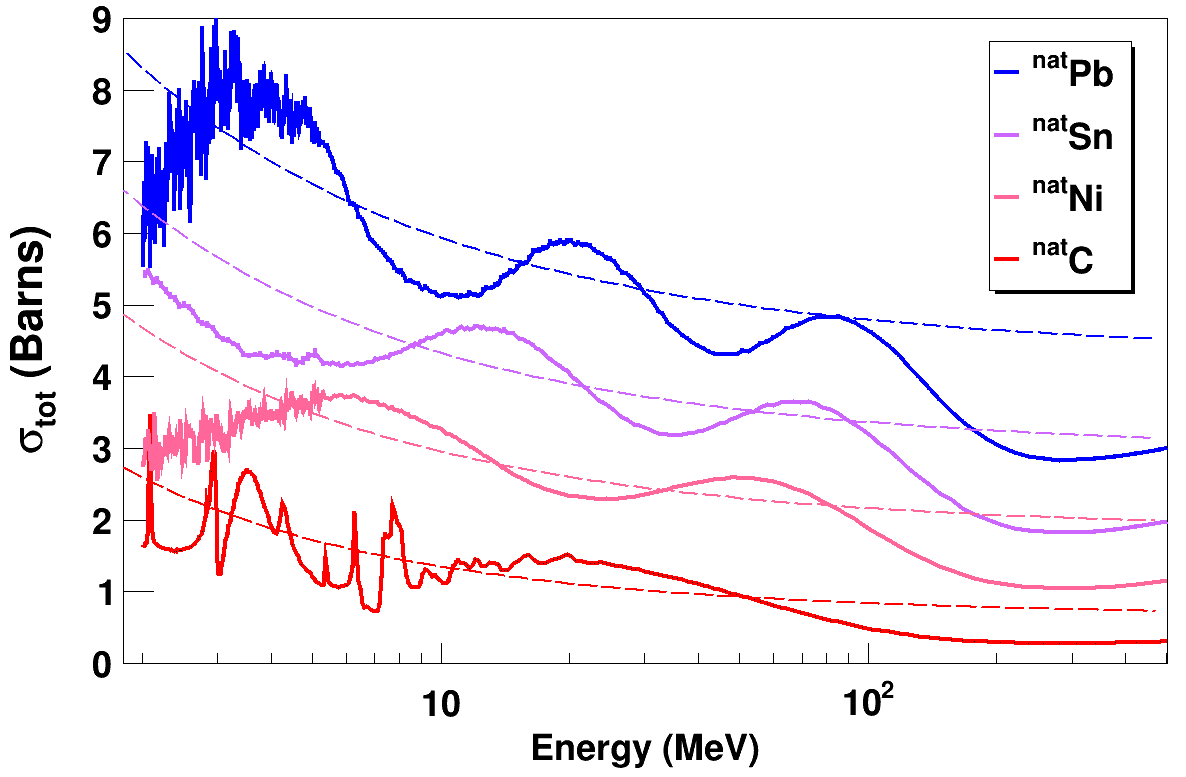
\includegraphics[width=0.9\textwidth]{figures/SASphereVsExperiment.png}
    \caption[Experimental neutron \tot\ data and strongly-absorbing-sphere predictions]
    {
        Experimental neutron \tot\ data on several natural samples (solid lines)
        from 2-500 \mega\electronvolt. The predictions of the crude strongly-absorbing-sphere
        model (Eq. \ref{SASAbsolute}) are shown as dashed lines. Resonance structures are
        clearly visible in the \cNat neutron \tot\ below 20 \mega\electronvolt.
    }
    \label{SASphereVsExperiment}
\end{figure}
These hallmark oscillations in the neutron \tot\ can be explained as the result
of a phase shift between 
neutron waves passing around the nucleus (unshifted) and waves passing
through the the nucleus, where they experience refraction
(illustrated in Fig. \ref{RamsauerPhaseShiftFigure}). This explanation was termed the ``nuclear 
Ramsauer effect'' by Peterson \cite{Peterson1962}, based on the analagous effect seen in 
electron scattering on noble gases.

Following Angeli \cite{Angeli1970}, these considerations can be incorporated by
imbuing the strongly-absorbing sphere relations (equation \ref{SASAbsolute}) with an additional sinusoidal term:
\begin{equation} \label{OscillatoryModel}
    \tot = 2\pi (R+\lambdabar)^{2}[1 - \rho \cos(\delta)]
\end{equation}
where $\rho = e^{-\operatorname{Im}(\Delta)}$, and $\delta =
\operatorname{Re}(\Delta)$, with $\Delta$ the phase difference between the wave traveling
around and traveling through the nucleus. Thus, the amplitude of the oscillation provides the 
elastic removal, or inelastic, phase shift and the period of oscillation
provides the elastic phase shift.
As can be seen from Eq. \ref{OscillatoryModel}, the large magnitude of the oscillations means that 
inelastic scattering (from $\operatorname{Im}(\Delta)$) accounts for only a small fraction of the 
total cross section, in turn implying a much larger mean free path for neutrons through the nucleus 
than would be expected in the absence of Pauli blocking \cite{Mohr1955}.

If the nucleus presents a spherical potential of radius $R$ and depth $U$, the total phase shift $\delta$ is:
\begin{equation} \label{phaseShift}
    \delta =
    \frac{\overline{C}\left(\left[{\frac{E+U}{E}}\right]^{\frac{1}{2}}-1\right)}{\lambdabar}
\end{equation}
where $\overline{C} = \frac{4}{3}R$ is the average chord length through the
sphere \cite{Angeli1970}. Rearranging Eq. \ref{phaseShift} in terms of A and E and
discarding leading constants yields:
\begin{equation}
    \delta \propto A^{\frac{1}{3}}\times\left(\sqrt{E+U}-\sqrt{E}\right)
\end{equation}
This form reveals an important relation: as A is increased, to maintain constant 
phase $\delta$, E must also increase \cite{Satchler1980, Peterson1962}. 
This is contrary to a typical resonance condition where an integer number of wavelengths
are fit inside a potential; in that case, to maintain constant phase as size is increased,
E must be decreased. Thus these \tot\ oscillations have been referred to as
``anti-resonances'' or ``echoes'' \cite{Satchler1980, McVoy1967}. It should be
noted that this simple Ramsauer picture is illustrative only, as it fails to
account for interference between the partial waves of the incident nucleon and
cannot be extrapolated to high energies without conspicuous deficiencies
\cite{Ahmad1973}.

A new type of nuclear model is thus at hand:
by replacing the intractable many-body problem
of the target nucleus by a complex, refractive potential, both elastic scattering (from the real 
part of the potential) and inelastic scattering (from the imaginary part) can be neatly 
explained. The existing mathematical machinery for calculating scattering of light from
refractive materials can then be repurposed for nuclear scattering, giving birth to
the ``optical model'' of the nucleus \cite{Feshbach1958, McVoy1967}.
Instead of a single central \gls{optical potential}, a series
of potential terms may be used,
centered on the nuclear surface and nuclear volume,
corresponding to differing physics thought to be relevant for these areas (much
as in the Droplet Model). Many comprehensive overviews of optical models are
available \cite{Dickhoff2018, Hodgson1971} that explore various potential forms
and connect optical models to other approaches.

\begin{figure}[tb]
    \centering
    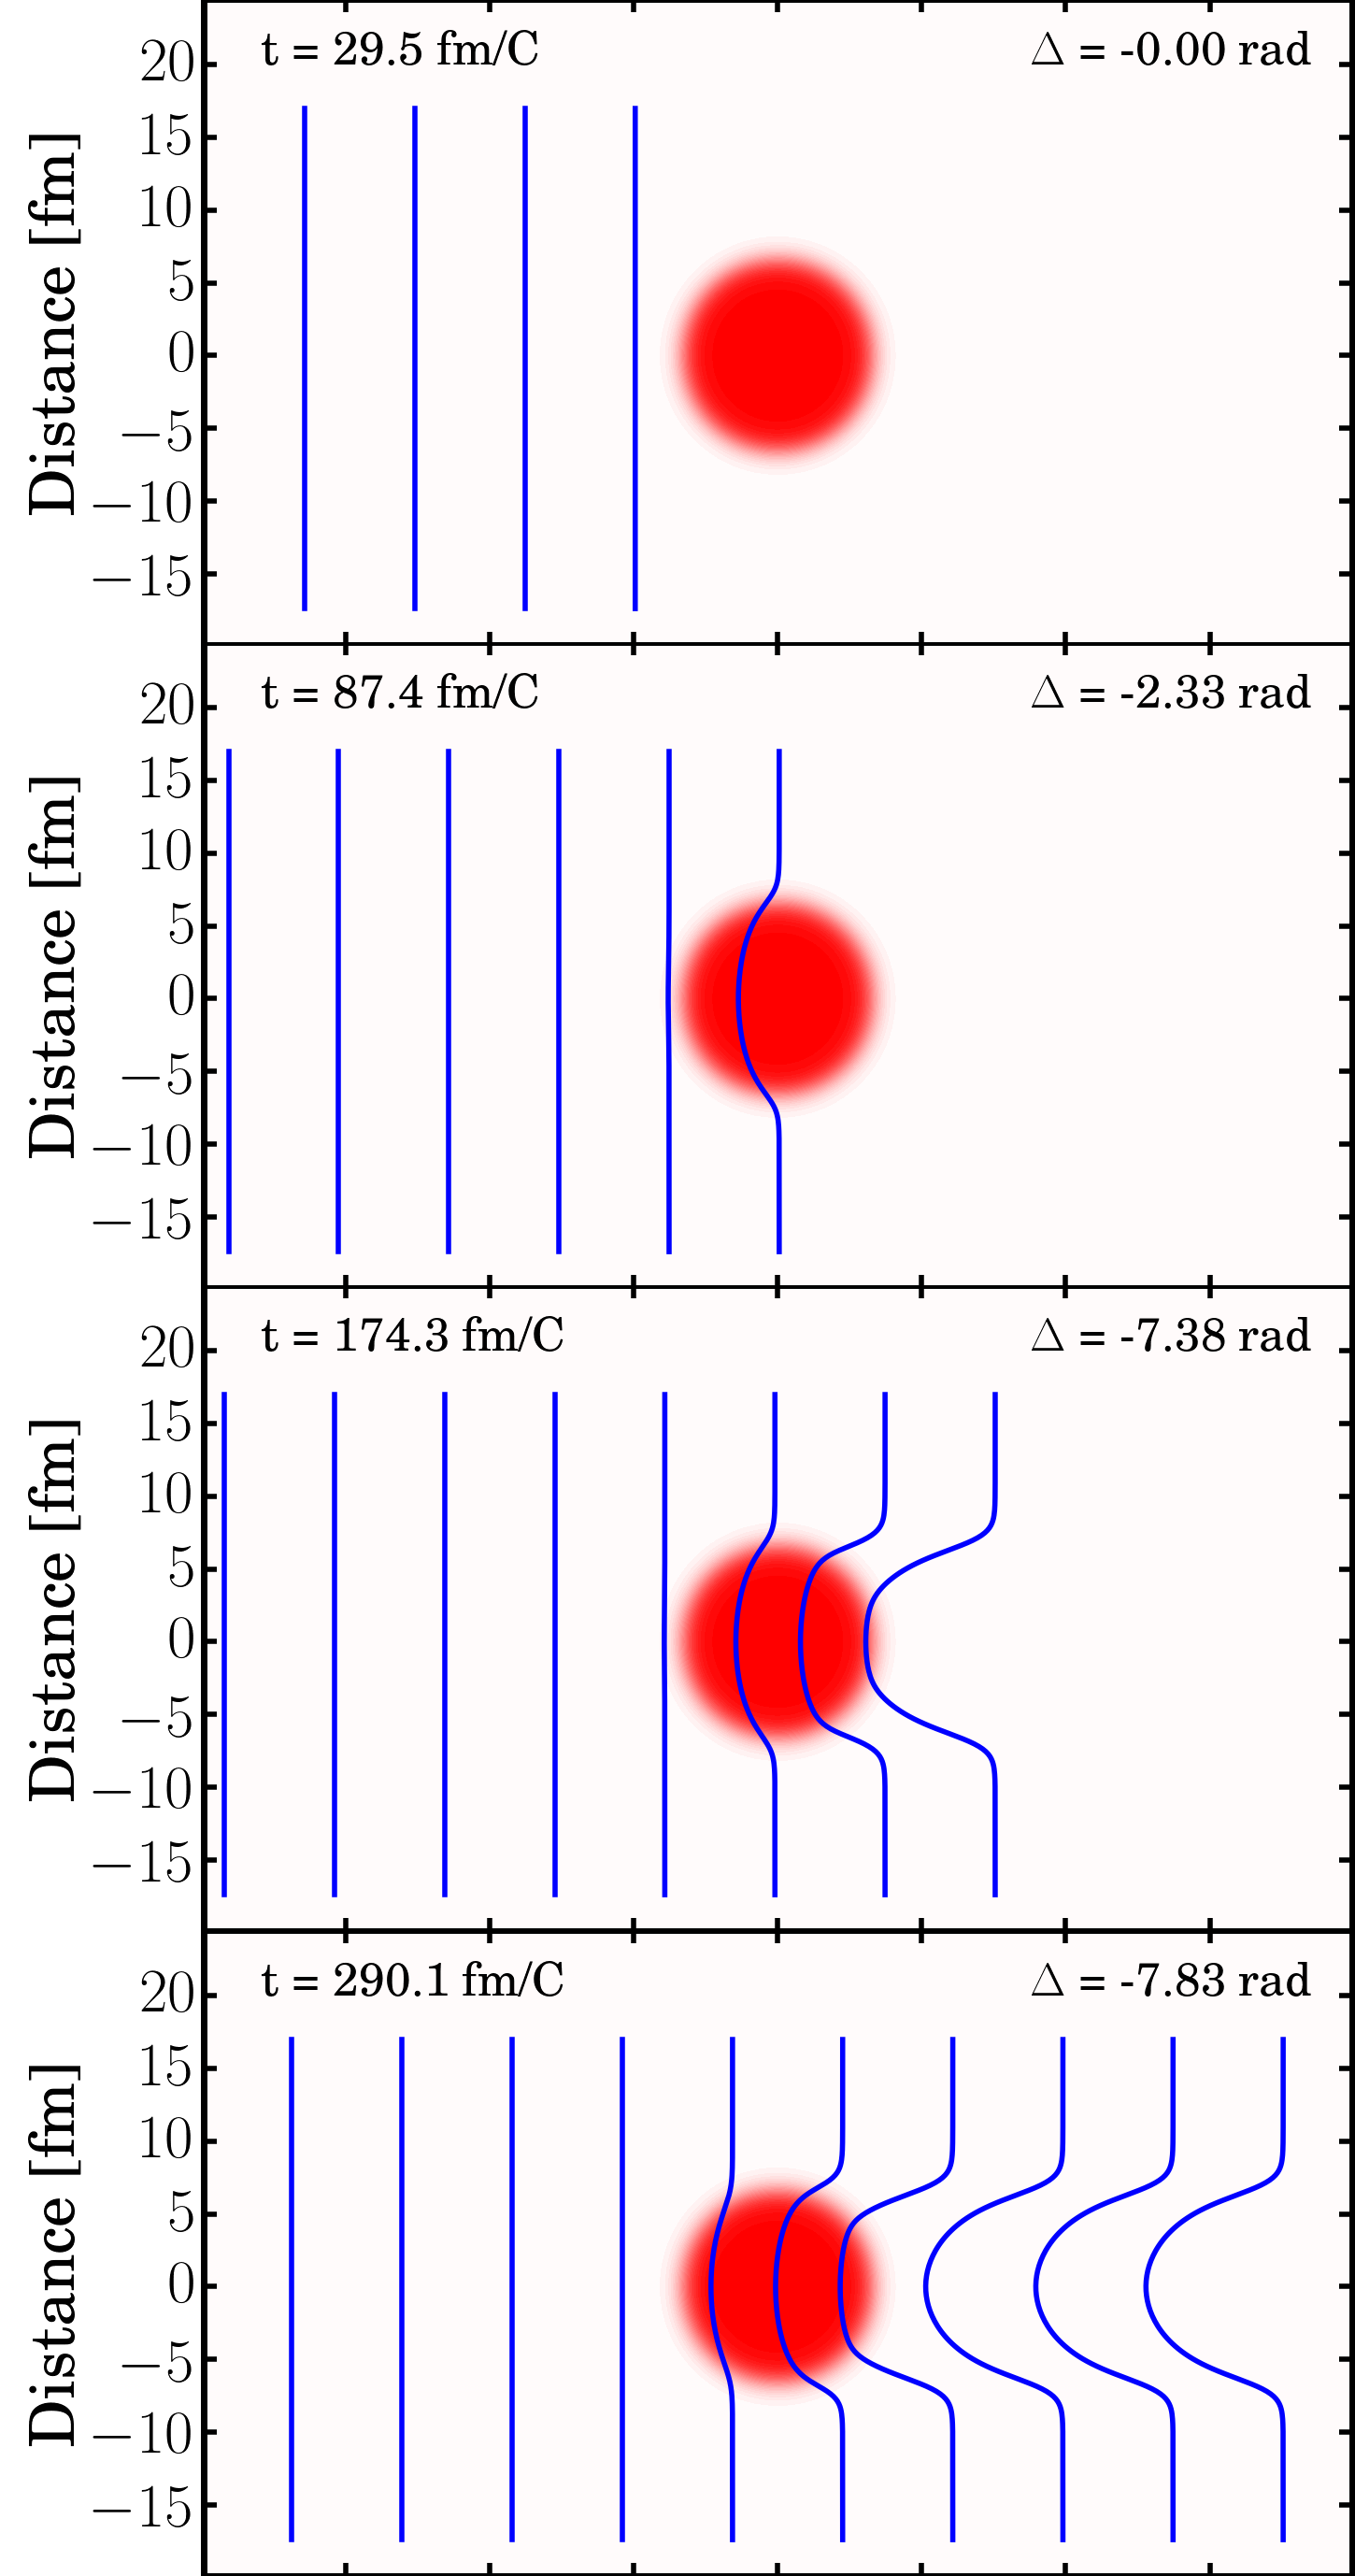
\includegraphics[height=0.7\textheight]{figures/phaseShiftStillsFigure.png}
    \caption[A illustration of the nuclear Ramsauer effect]
    {
        A neutron wave train (series of
        blue lines) impinges from the left on a real Woods-Saxon
        potential centered at the origin (diffuse red circle). The potential
        refracts the neutron wave,
        retarding the phase of the wavefront as it passes through the
        potential. After escaping the potential, a phase difference $\Delta$ between
        the wave component passing \textit{around} and \textit{through the center}
        of the potential persists, resulting in scattering.
        For the leading wavefront in the wave train, $\Delta$ is indicated in
        the top right-hand corner of each panel. A differential version of
        Eq. \ref{phaseShift} is used to
        calculate the phase shift for each step. In this figure, the neutron
        energy $E_{n}$ = 14 \mega\electronvolt\ and nuclear mass $A$ = 25. For the Woods-Saxon potential,
        we used a potential depth $U$ = 42.8 \mega\electronvolt\ (following Angeli and Csikai's analysis
        of \tot\ data at 14 \mega\electronvolt\ \cite{Angeli1970}), with nuclear radius $R = 
        r_{0}A^{\frac{1}{3}}$, $r_{0}$ = 1.4 fm, and a diffuseness parameter
        $a$ of 0.5 fm.
    }
    \label{RamsauerPhaseShiftFigure}
\end{figure}

Global OMs have been developed to simultaneously reproduce single nucleon, heavy ion,
and other hadron scattering data on targets across the chart of nuclides up to several
hundred \mega\electronvolt\ \cite{CH89, KoningDelaroche}. Because the proton-proton,
proton-neutron, and neutron-neutron scattering cross sections
are not identical, OM potentials are expected to differ for protons and
neutrons. Isoscalar terms, which respect isospin symmetry and thus treat protons and neutrons 
identically, account for most of the observed scattering, but do not include
the asymmetry-\textit{dependent} interactions known to exist between
nucleons, such as charged meson exchange.
Thus isovector and isotensor terms,
which depend on the difference between the proton and neutron density
distributions in the nucleus, are needed. As experimental facilities like
the Facility for Radioactive Isotope Beams (FRIB) come online and produce
extremely asymmetric nuclei, knowing the asymmetry-dependence of optical
potentials will become increasingly important for predicting nucleon scattering on
exotic nuclei. Isovector considerations are not unique to full-blown optical
models and can be introduced to a simpler Ramsauer-like models as well. For example, building
on the addition of spin-spin terms a Ramsauer model by Gould et al. \cite{Gould1986},
Anderson and Grimes added an explicit isovector term to analyzing isotone and isotope shifts in 
neutron total cross sections \cite{Anderson1990}.
They concluded that ``although [their] model may give
semiquantitative agreement with some aspects of the data, optical-model
calculations should be used for quantitative comparison''.

Despite their excellent reproduction of experimental data,
OMs involve the interaction of
many sometimes-opaque parameters with many incident
partial waves, blurring the intuitive picture of the underlying physics.
OMs are unabashedly phenomenogical so a wide variety of
experimental data types and energies are required to constrain the potential,
so when data are absent, model predictions are poor. Without a clearer connection to formal
many-body methods, the empiricism of optical models does clarify the connection between nuclear
reactions and nuclear structure. A major step forward was taken by Mahaux and Sartor
\cite{Mahaux1991}, who linked the nucleon self-energy to the \gls{optical potential} by means of a
dispersion relation, allowing for a more-direct comparison between scattering data and mean-field nuclear
structure calculations. We employ a descendant of their
dispersive optical model, generalized to include a
fully non-local potential, to treat nuclear structure and reactions on the same
footing.

A long-standing difficulty in optical-model analyses is in constraining the isovector dependence
of the real and imaginary parts of the potential \cite{Holt16, Anderson1990}. Improving constraints on the
isovector terms in particular requires data
on asymmetric nuclei, preferably on highly-asymmetric nuclei or isotopic chains,
where the imbalance of protons and neutrons makes any isovector effects most visible. The isovector
strength of the nuclear potential is directly connected to a host of open problems in nuclear physics,
including fixing the density-dependence of the symmetry energy, $L$, locating the
neutron dripline, and understanding how high-momentum content is distributed between neutrons and
protons. Making progress in this area requires improved experimental data sets
and is the main concern of the following section.

\section{Relevant Experimental Nuclear Data}

\subsection{Nucleon scattering data}
Elastic nucleon scattering cross sections, especially with protons, comprise the most extensively-measured
sector of experimental scattering databases. The EXFOR experimental reaction database
\cite{EXFORDatabase} contains thousands of proton and neutron
differential elastic scattering and analyzing
power data sets between 1-300 \mega\electronvolt, the domain relevant for this work. Optical model fits
to these data, both regional and global \cite{CH89, KoningDelaroche}, have helped
constrain nuclear radii, the strength of the spin-orbit coupling,
and revealed the importance of an imaginary spin-orbit term.

Inelastic nucleon scattering data are more difficult to collect experimentally and much sparser in
the literature record. By helping fix the strength and energy-dependence of the absorptive component
of the nuclear potential, inelastic data serve a complementary role to elastic
data.
%The was pointed out by Finlay et al. in 1993:
%\begin{displayquote}
%    ``Above about 200 \mega\electronvolt, an impulse approximation might be expected to
%    give a good description of the data, while at lower energy Pauli blocking and
%    medium effects must be included. Phenomenologically, the imaginary term in
%    the optical potential increases rapidly, while the real term is thought to
%    pass through zero \cite{Finlay1993}.''
%\end{displayquote}
\noindent
Isotopically-resolved data is particularly valuable for constraining nuclear
models, as it avoids averaging over multiple isotopes naturally present in many elemental samples.
Unfortunately, many pure isotopes are extremely expensive ($>$\$10,000 per gram) to
separate, putting them out of reach for all but the most well-funded experiments.
Indeed, as late as 1988, only a handful of neutron \tot\ measurement campaigns
on multiple samples had been conducted, most of them elemental, not isotopic
\cite{BarnBook1988}.

Figs. \ref{TCSChart} and \ref{RCSChart} illustrate the status of isotopically-resolved inelastic
nucleon scattering data in the EXFOR nuclear reaction database as of 2019.
Except for light isotopes and a few security-related actinides, coverage is
sparse and has changed little since the early 2000s. The single notable
exception is the triplet of $^{182,184.186}$W data sets from 5-560 \mega\electronvolt\ of \cite{Dietrich2003}, 
mentioned in the previous section. Isotopic \textit{proton} \rxn\ measurements over
a broad energy range are particularly lacking due to the paucity of suitable
accelerators and the subtlety of such a measurement. 
Both high-energy ($>$100 \mega\electronvolt) neutron \tot\ and proton \rxn\ data are useful for
understanding the asymmetry-dependence of the imaginary strength of the nuclear potential.
In this work, we focus on isotopically-resolved neutron scattering, which
is easier to measure and, when combined with proton \textit{elastic} cross sections,
also provides information on the asymmetry-dependence of the real part of the nuclear potential.

\begin{sidewaysfigure}
    \centering
    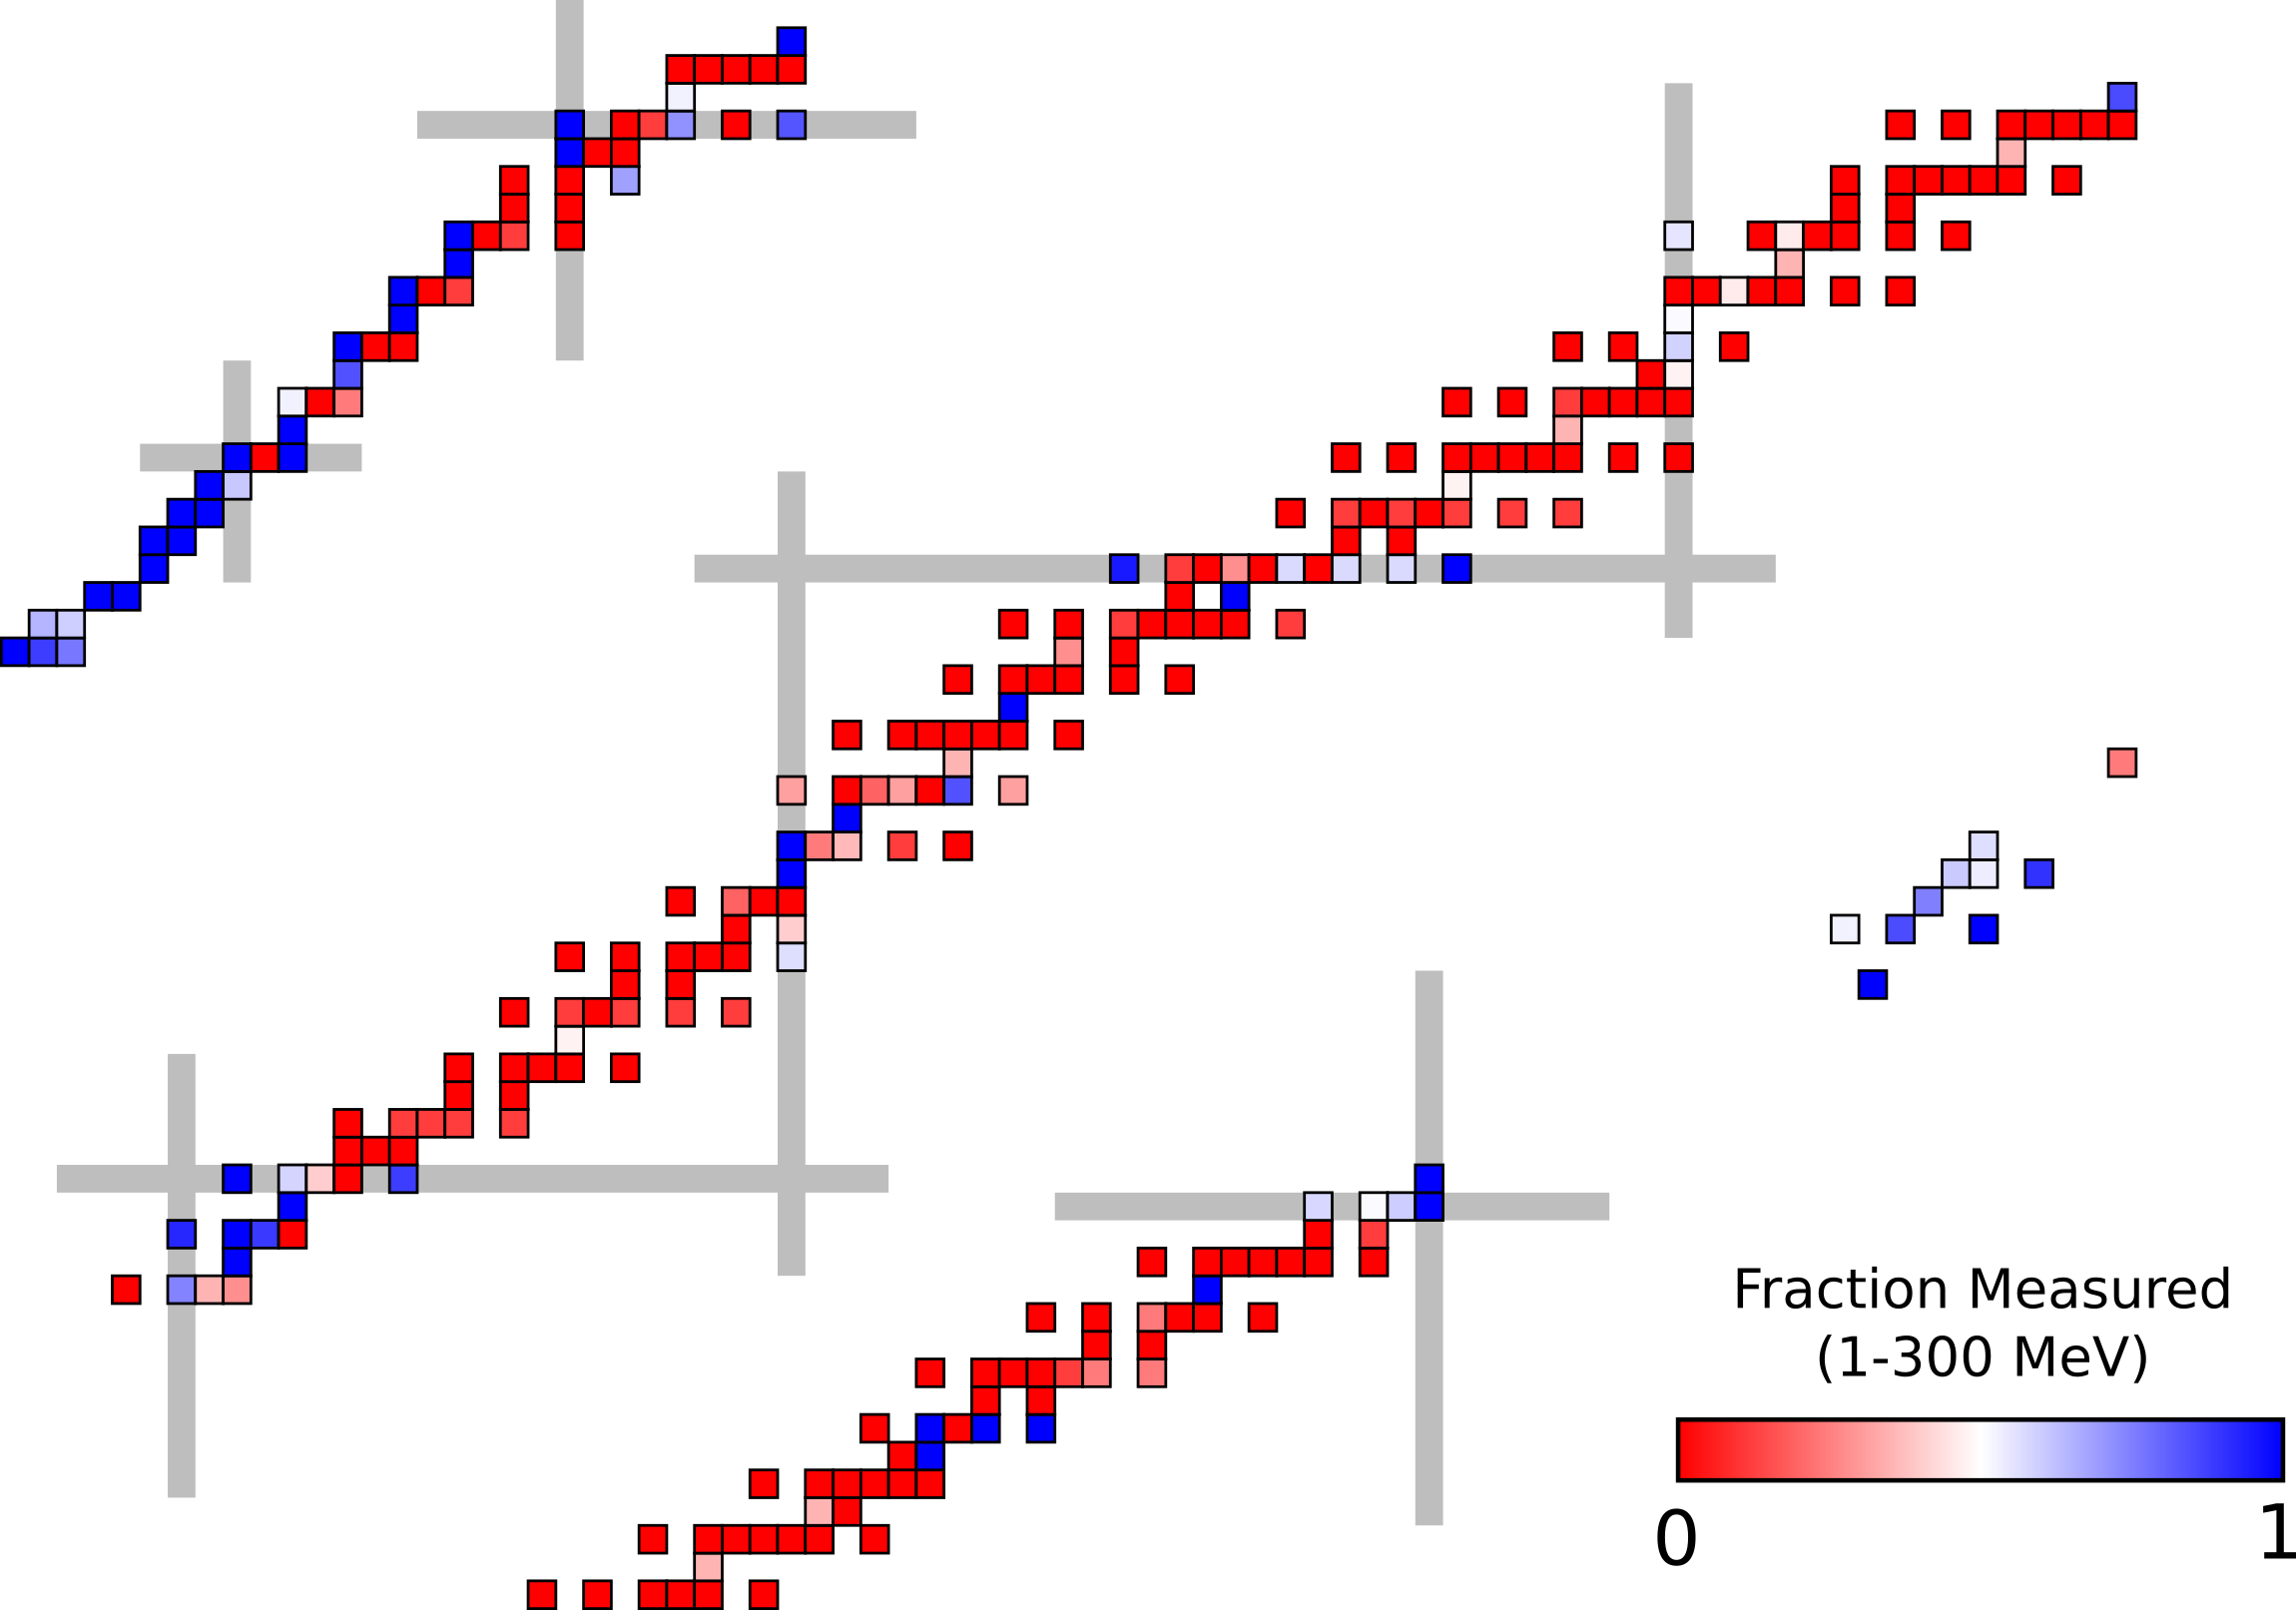
\includegraphics[width=0.9\textwidth]{figures/TCSChart.png}
    \caption[Landscape of existing neutron \tot\ data in 2019]
    {Isotopes are color-coded by the amount of neutron \tot\ data available in the EXFOR nuclear
        reaction database from 1-300 \mega\electronvolt, as accessed in 2018 and 2019. If data exists thoughout the
        1-300 \mega\electronvolt\ range, the isotope
        is colored blue. If no data exists, the isotope is colored red. For
        isotopes with partial coverage in this range, color varies by the degree
        of coverage. Except for the lightest
        isotopes (O and below), a few security-related actinides, there is almost no coverage
        throughout the nuclear chart. Our newly-measured results on \oSixEight, \niEightFour,
        \rhThree, and \snTwelveFour\ are included, as are a previous experiment
        by our group on \caAughtEight \cite{Shane2010}.
    }
    \label{TCSChart}
\end{sidewaysfigure}

\begin{sidewaysfigure}
    \centering
    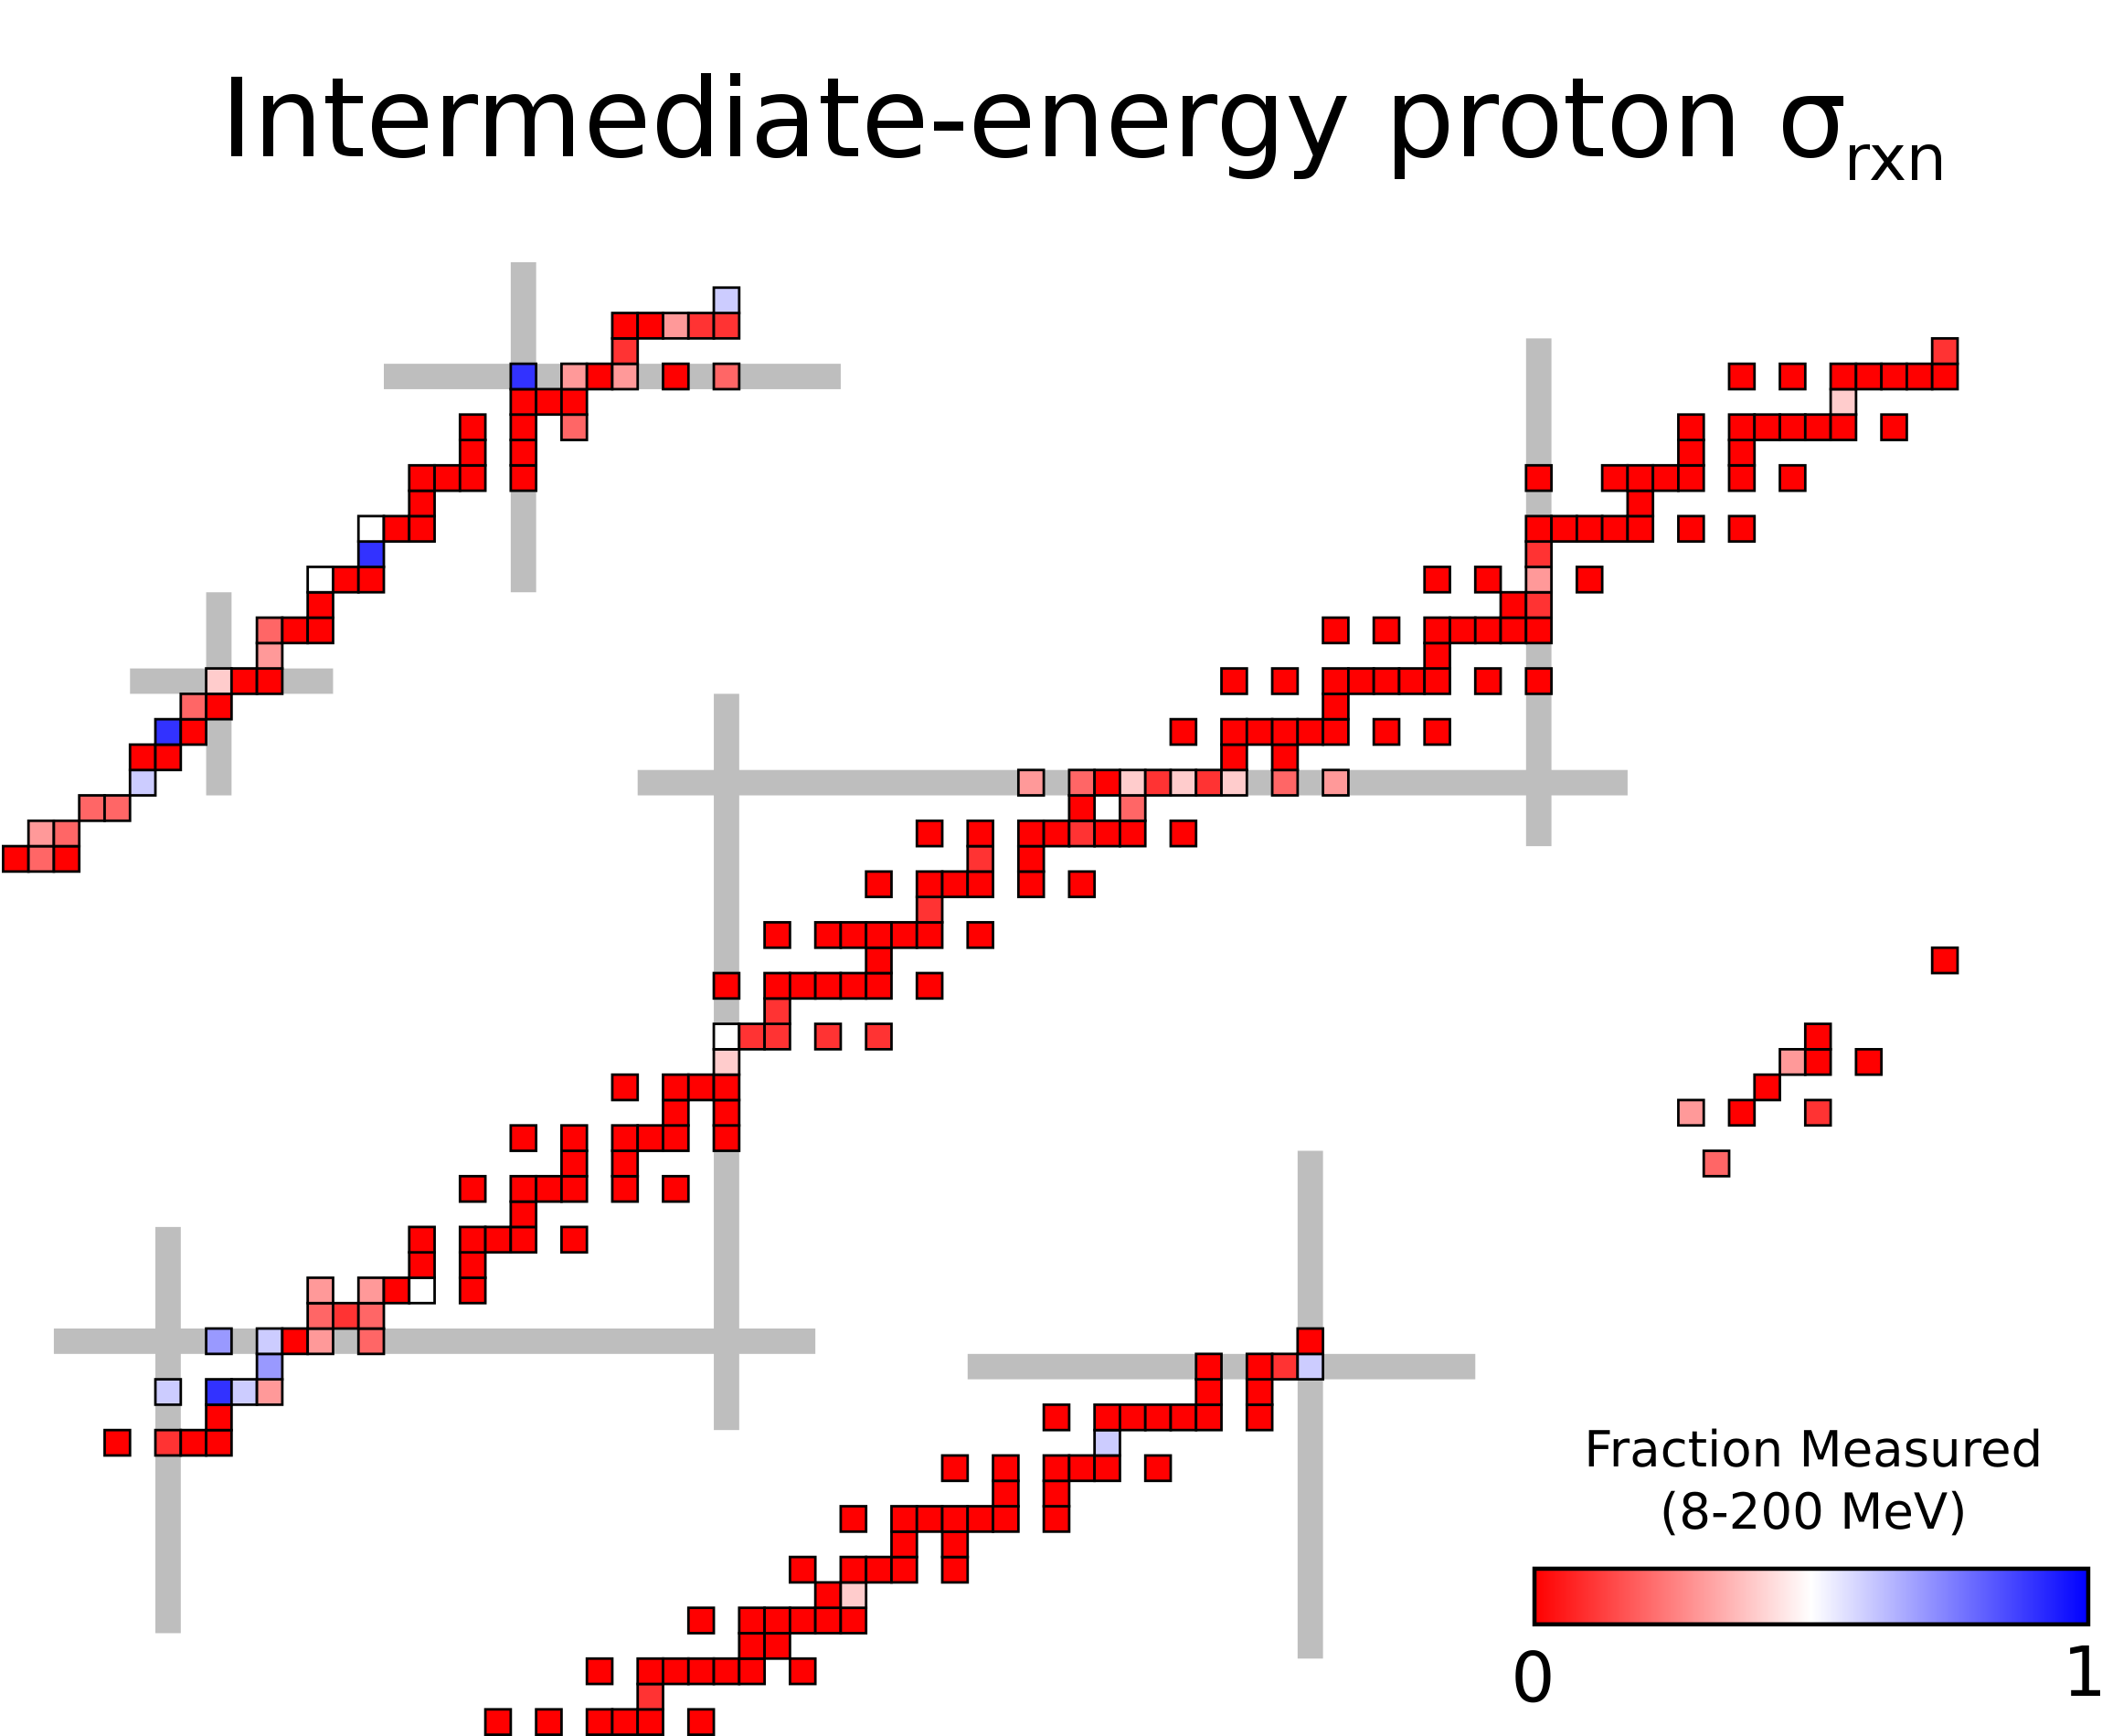
\includegraphics[width=0.9\textwidth]{figures/RCSChart.png}
    \caption[Landscape of existing proton \rxn\ data in 2019]
    {Isotopes are color-coded by the amount of neutron \tot\ data available in the EXFOR nuclear
        reaction database from 1-300 \mega\electronvolt, as accessed in 2018 and 2019. If data exists thoughout the 1-300 \mega\electronvolt\ range, the isotope
        is colored blue. If no data exists, the isotope is colored red. For
        isotopes with partial coverage in this range, color varies by the degree
        of coverage. Almost no nuclei have experimental coverage throughout this energy
        range, a testament to the difficulty of proton \rxn\ measurements.}
    \label{RCSChart}
\end{sidewaysfigure}

In the last few decades, a smattering of isotope-chain neutron total cross section
analyses have been carried out \cite{Mukhopadhyay2011, Anderson1990, Camarda1984}. The most sophisticated
was conducted by Dietrich et al.\cite{Dietrich2003},
using new data they measured on the $^{182,184,186}$W isotope chain (quite noticeable in Fig.
\ref{TCSChart}). In their study, an expanded Ramsauer-type model performed quite well at reproducing the relative 
difference between $^{186}$W and $^{182}$W, apart from a
phase mismatch - but only when the isovector components they introduced in the
Ramsauer model are \textit{suppressed} (see Fig. \ref{Dietrich2003_Ramsauer}). Despite the
dubiousness of ignoring isospin, the resulting Ramsauer model
agrees better with the experimental data than does the Ohio global optical 
potential \cite{Rapaport1979}, shown in Fig. \ref{Dietrich2003_Ohio}.

\begin{figure}[tb]
    \centering
    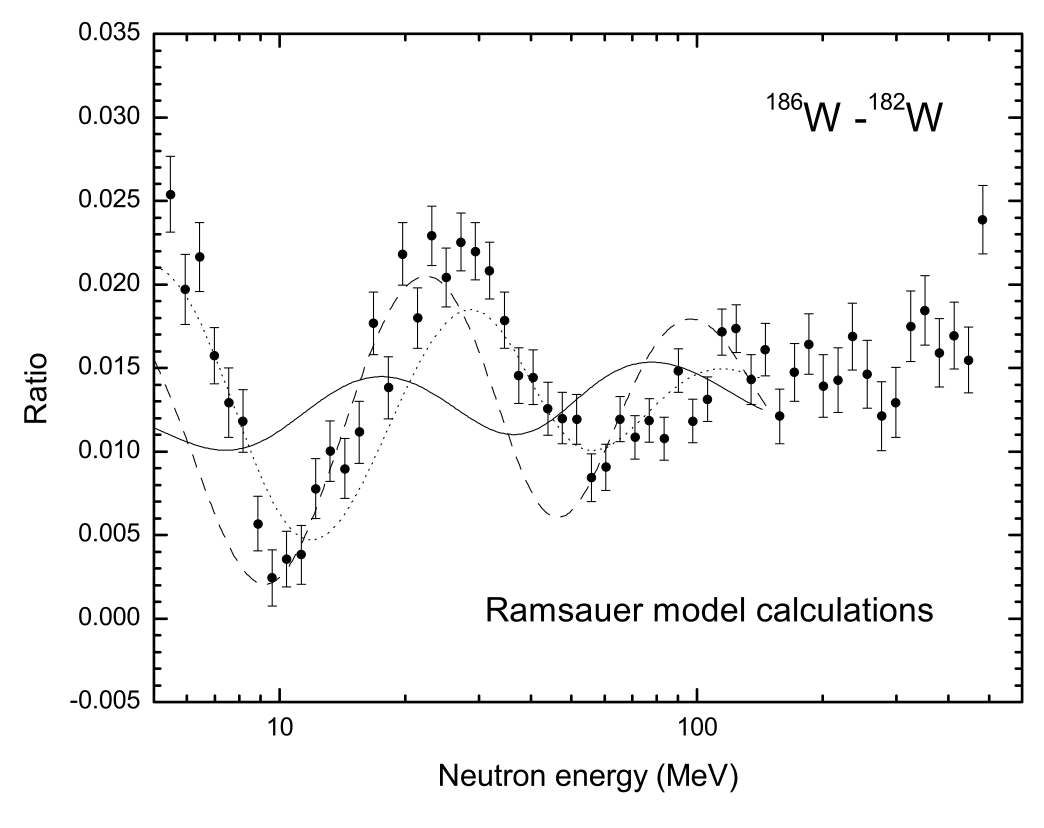
\includegraphics[width=0.8\textwidth]{figures/Dietrich2003_RamsauerPotential.png}
    \caption[$^{186}$W-$^{182}$W neutron \tot\ relative difference and
    Ramsauer model predictions]
    {
        $^{186}$W-$^{182}$W neutron \tot\ relative difference and
        Ramsauer model predictions. Figure from \cite{Dietrich2003}.
        If the standard isovector strength from
        optical-model treatments is used to dictate the Ramsauer isovector
        dependence (solid line), the model performs more poorly against the experimental
        data. When the isovector strength is suppressed, the correspondence to data improves (dashed
        line).
    }
    \label{Dietrich2003_Ramsauer}
\end{figure}

\begin{figure}[tb]
    \centering
    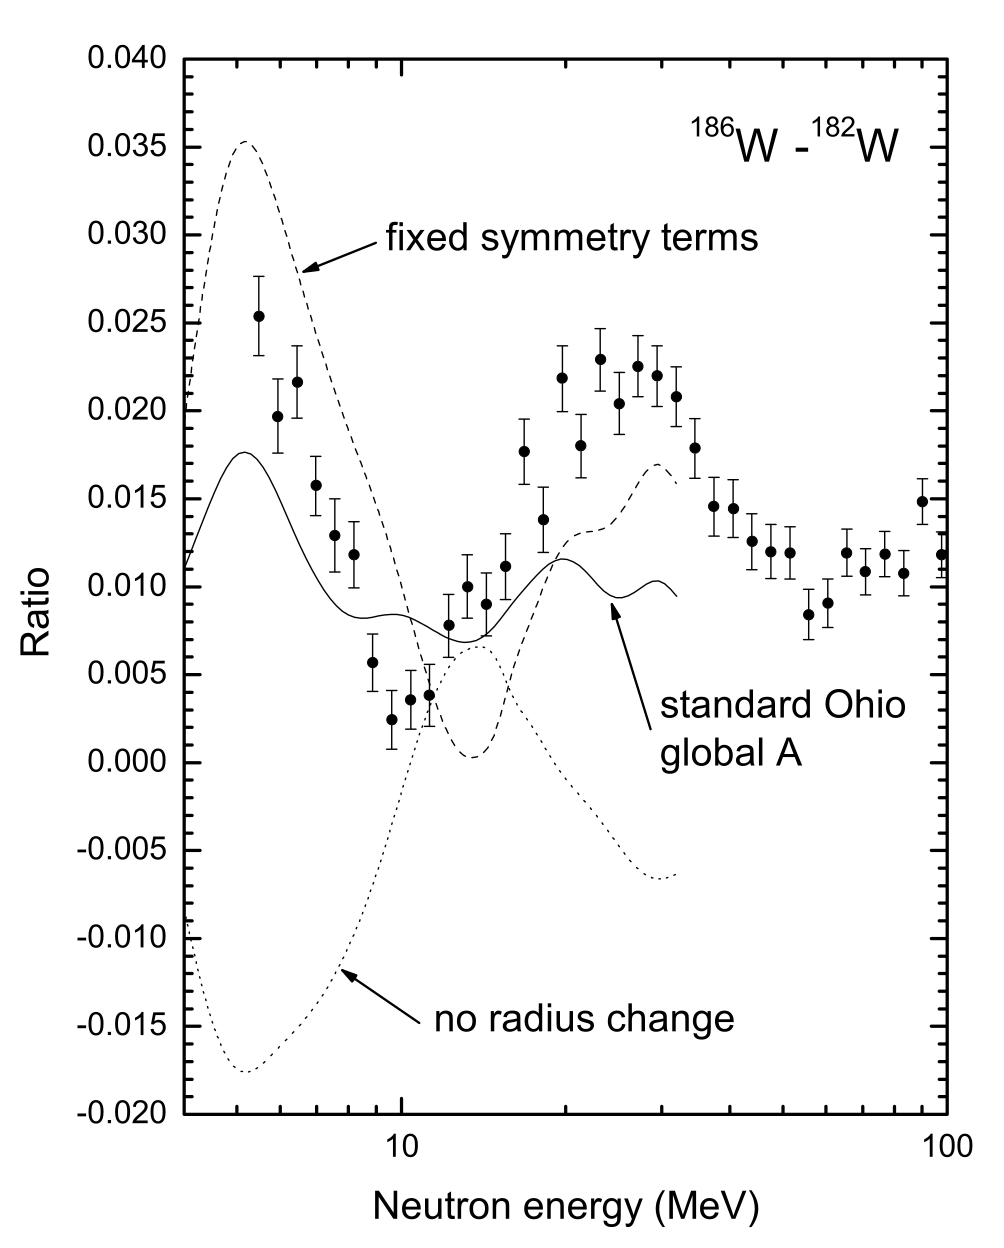
\includegraphics[width=0.6\textwidth]{figures/Dietrich2003_OhioPotential.png}
    \caption[$^{186}$W-$^{182}$W neutron \tot\ relative difference and
    Ohio global optical model predictions]
    {
        $^{186}$W-$^{182}$W neutron \tot\ relative difference and
        Ohio global optical potential predictions. Figure from \cite{Dietrich2003}.
    }
    \label{Dietrich2003_Ohio}
\end{figure}

The authors also performed phenomenological coupled-channel calculations
based on a dispersive optical model formalism
\cite{Mahaux1991} that showed similar behavior: it gave good agreement with the
experimental \tot\ relative differences, but only when isovector terms in the calculations
were explicitly \textit{neglected}. As the
authors point out, it is quite puzzling that ``good agreement with the
experimental data can be obtained at the expense of an incorrect physical
picture''.
Of the models they tested, only a deformed, semimicroscopic
optical model potential (SMOMP),
obtained by folding an energy- and density-dependent optical model potential from nuclear matter 
calculations over the deformed nuclear densities, was capable of satisfactorily describing the
\tot\ isotope shift in W. From this case study on W isotopes, several followup questions
are apparent: is a microscopic knowledge of the proton and neutron matter
densities important for reproducing the neutron \tot\ across an isotope
chain? More fundamentally, what terms in an optical potential are the neutron
\tot\ cross sections sensitive to, and are neutron \tot\ data connected to
structural (i.e., bound-state) information in a consistent, transparent way?

Answers to these questions hinge on the availability well-measured 
isotopic neutron \tot\ data sets across a broad energy range. Indeed, the
\caAughtEight\ neutron \tot\ data collected by our group at LANSCE in 2009, in
part inspired by the W measurements of \cite{Dietrich2003},
provided grist for a non-local Dispersive Optical Model (DOM) analysis in 2015
\cite{MahzoonPhDThesis}. This non-local analysis revealed connections
between the asymmetry-dependence of single-particle occupation numbers
and high-energy scattering data.
Providing experimental data on key nuclei, in particular for use with the \gls{DOM},
is a primary motivation for the isotopically-resolved neutron \tot\ and \el\
results presented in this work. These new data are analyzed in Chapter \ref{DOMResults} 
with an improved non-local DOM capable of fits to data on even-even nuclei. Details on our DOM
implementation are presented in chapter \ref{DOMFormalism}. 

\subsection{Nuclear Masses, Matter Radii, and Charge Radii}
The mass and spatial extent of a nucleus are two of its most fundamental
properties. Of all experimental data, nuclear masses are known to the highest
precision, up to ten significant digits \cite{AME2016}. Connecting masses and
radii is a central design of the Liquid Drop Model and many other theoretical
treatments over the last century (e.g., Hartree-Fock-BCS treatment of 700 nuclei to calculate 
proton and neutron RMS radii \cite{Angeli1980}). Extracting nuclear radii from optical
models have been an active area of research for over fifty years \cite{Jackson1974}.

Experimentally, a variety of techniques are available to probe the nuclear
charge density distribution. On stable nuclei, x-ray energies from muonic atoms
\cite{Fricke2004} are sensitive to deviations of the nuclear charge
distribution from sphericity, and elastic electron
scattering data can be used, after Fourier transform, provide the full nuclear
charge density profile at spatial resolutions between $\frac{2\pi}{q_{min}}$ and
$\frac{2\pi}{q_{max}}$, where $q$ is the momentum transfer associated with the
elastic scattering \cite{DeVries1987}.
On unstable nuclei, collinear laser spectroscopy \cite{Miller2019},
uses small shifts in electronic levels to extract
the difference in RMS radii ($\delta_{RMS}$) of the charge
distributions along an isotope chain, the so-called ``isotope shift''.
The isotope shift is shown for the even-A Sn isotopes in Fig.
\ref{SnIsotopeShift} \cite{Anselment1986}.
\begin{figure}[tb]
    \centering
    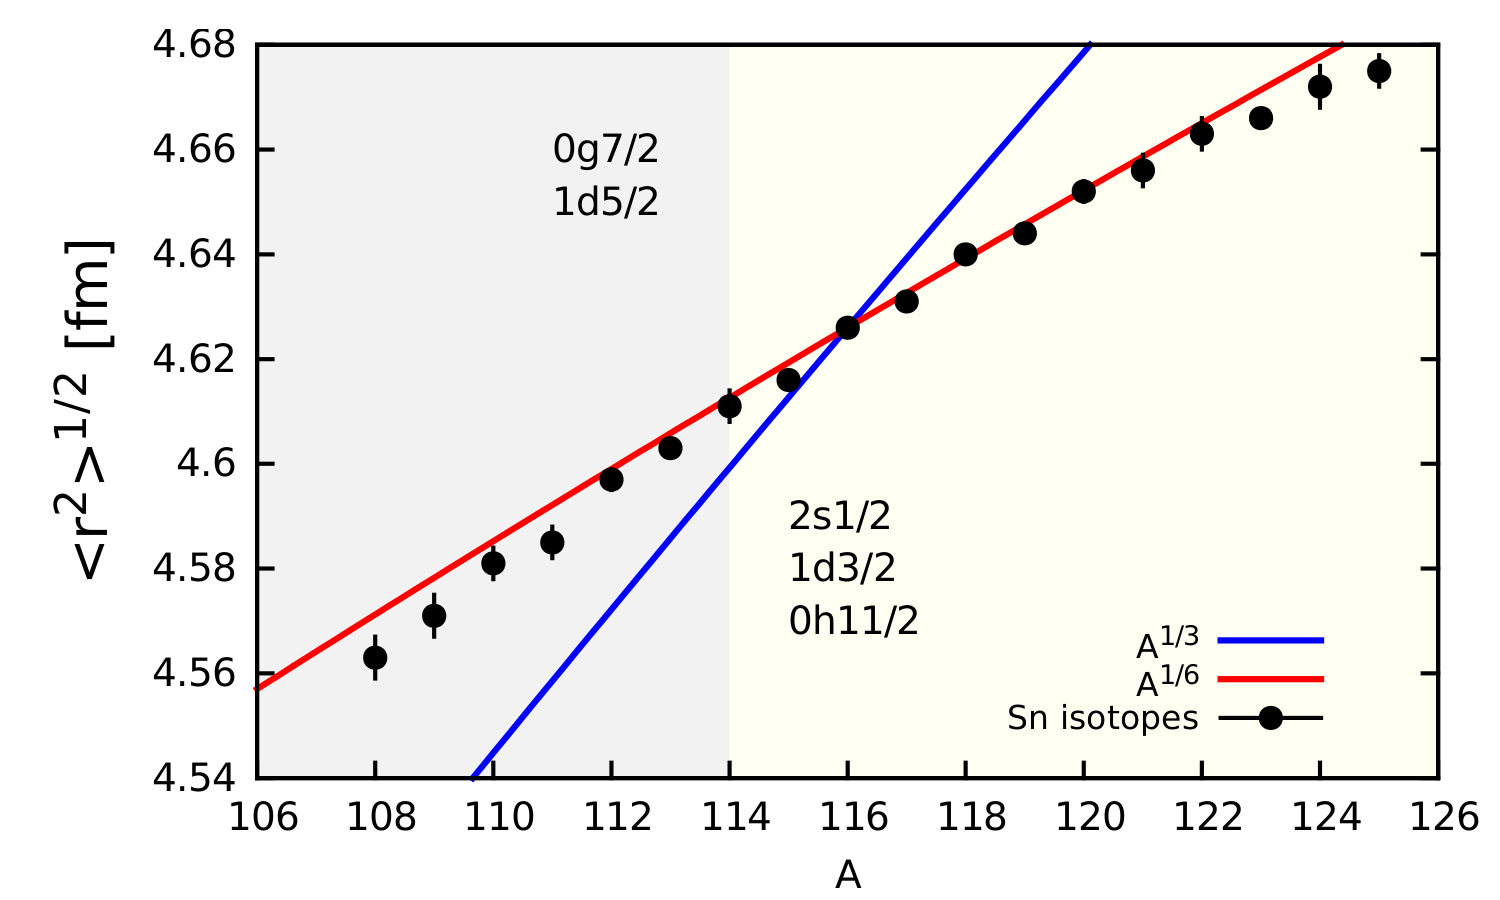
\includegraphics[width=0.9\textwidth]{figures/SnIsotopeRMSRadii.png}
    \caption[Root-mean-squared charge radii of Sn isotopes]
    {
        Root-mean-squared (RMS) charge radii in Sn isotopes.
        The A=106-114 region and A=114-116 region are shaded and labeled
    indicating the expected single-particle occupation of the valence neutrons.
    An isoscalar treatment that only accounts for size scaling predicts an
    A$^{\frac{1}{3}}$ slope as neutrons are added, but the data show a nearly-linear
A$^{\frac{1}{6}}$ slope instead. The slope of the isotope shift is connected to the symmetry energy
and its density dependence. Data from Anselment et al. \cite{Anselment1986}}.
    \label{SnIsotopeShift}
\end{figure}
It has long been clear that the 
isotope shift is critically connected to the neutron and proton matter distributions.
The difference in RMS radii between the protons and neutron point distributions
(i.e., not including the finite size of the protons and neutrons) is commonly referred to as the 
``neutron skin''  \cite{Otten1989} and was first identified as an important
nuclear quantity by Wilkinson over fifty years ago \cite{Wilkinson1967}.
In a Droplet Model picture, the slope of the isotope shift is linked to the symmetry energy $J$, 
density dependence of the symmetry energy
$L$, and surface stiffness coefficient $Q$\footnotemark, the same bulk quantities that determine
neutron-skin thickness \cite{MyersAndSwiatecki, Berdichevsky1988}.
\footnotetext{
    In \cite{MyersAndSwiatecki}, the $J$-, $L$-, and $Q$-dependent contributions to the
    binding energy are:
    \begin{equation*}
        \begin{split}
            E(N,Z;shape) & =
            [J\bar{\delta}^{2}-\frac{1}{2}K\bar{\epsilon}^{2}
            +\frac{1}{2}M\bar{\delta}^{4}]A\\
            & + \frac{9}{4}(J^{2}/Q)\bar{\delta}^{2}A^{\frac{2}{3}}B_{s}
            + CC(J,Q)
        \end{split}
    \end{equation*}

    \noindent
    where $\bar{\delta}$ and $\bar{\epsilon}$ of Eq.
    \ref{DropletIndependentQuantities} are fully parameterized as: 
    \begin{equation*}
        \begin{split}
            \bar{\delta} & = I+\frac{3}{16}(c_{1}/Q)ZA^{-\frac{2}{3}}B_{v}]
            /[1+\frac{9}{4}(J/Q)A^{-\frac{1}{3}}B_{s}]\\
            \bar{\epsilon} & = [-2a_{2}A^{-{\frac{1}{3}}}B_{s}+L\bar{\delta}^{2}
            +c_{1}Z^{2}A^{-\frac{4}{3}}B_{c}]/K
        \end{split}
    \end{equation*}
    
    \noindent
    In these equations, $K$ is the compressibility coefficient, $M$
    accounts for anharmonicity of the binding-energy dependence on $\bar{\delta}$,
    and $B_{s}$ accounts for shape dependence of the surface energy. $CC(J,Q)$ are
    corrections to the Coulomb term associated with deformation. The quantity
    $\frac{9}{4}(J^{2}/Q)\bar{\delta}^{2}$ is the correction to the binding
    energy from excess neutrons accumulating on the nuclear surface in neutron-rich
    systems (i.e., neutron skin formation).
}
\noindent
Without addition experimental constraints, the $J$, $L$, and $Q$ parameters form an
underdetermined system from which unique values cannot be recovered, even if the
consensus value of $J \approx$ 30 \mega\electronvolt\ is used to reduce the parameter space.
As was already pointed out 50 years ago by Myers \cite{Myers1969},
the single-particle configuration of a given nucleus may have a significant
effect on the formation and size of such a skin.

Charge radius measurements have
become sufficiently precise that models can no longer equate the proton matter
distribution and the charge distribution; the non-uniform charge distributions of the
proton and neutron must be accounted for as well. Constraining the neutron matter
distribution experimentally is extremely difficult, as neutrons do not interact
Coulombically with the electron and muonic probes used to determine the charge
distribution. An on-going, multi-year
experimental effort at Jefferson Laboratory aims to measure the \caEight\ and
\pbEight\ neutron and proton matter distributions directly using parity-violating electron
scattering, taking advantage of different weak charges of the proton and neutron
\cite{Horowitz2014}. The neutron skins of these and other neutron-rich nuclei
are of immense theoretical and astrophysical interest, as they are closely
correlated with the density-dependence of the symmetry energy, essential
for the neutron star equation-of-state, and with many other bulk properties of
nuclei, including the electric-dipole-polarizability (EDP) and the location of the
pygmy and giant dipole resonances (PDR and GDR)
\cite{Vinas2014, Brown2000, Fattoyev2012, Piekarewicz2012, Zhang2018}.
Constraining $L$ using these asymmetry-dependent 
properties is quite challenging: the properties of highly-asymmetric nuclei are
most closely correlated with $L$, but harder to measure experimentally, and the
properties of low-asymmetry nuclei are much more weakly correlated with $L$.
One of the chief goals of the Dispersive Optical
Model (detailed in Chapter \ref{DOMFormalism}) is to extract well-constrained values for the 
neutron skin thickness on a variety of nuclei (shown in Chapter
\ref{DOMResults}). By judiciously applying all available scattering and bound-state
data in the DOM approach, we hope to test the assertion
that the EDP, GDR location, neutron skin, and $L$ are as tightly correlated as
it appears from mean-field models.

\section{Motivation, Scope, and Dissertation Outline}
Improved isotopically-resolved neutron scattering data are an essential ingredient
for better nuclear reaction models and to test the asymmetry-dependence of the
nuclear potential. The results of our campaign to collect these valuable
\tot\ and \el\ data sets on cornerstone nuclei form the backbone of this dissertation.
In addition to these experimental results, a suite of Dispersive Optical Model analyses that 
incorporates these new data is presented. From the DOM potentials, a variety of asymmetry-dependent 
nuclear-structure quantities, including neutron skins and relative momentum
content, are extracted.

An overview of neutron \tot\ experimental considerations, the details of our 
\tot\ experiment, and analysis for our isotopically-resolved \tot\ measurements
on \oSixEight, \niEightFour, \rhThree, and \snTwelveFour\ are detailed in 
Chapters \ref{TCSExperiment} and \ref{TCSAnalysis}. Similarly, our elastic scattering measurements 
on \snTwelveFour\ are presented in Chapters \ref{ECSExperiment} and \ref{ECSAnalysis}. A brief 
summary of the Dispersive Optical Model formalism is
given in Chapter \ref{DOMFormalism} and the results from our DOM fits of \oSixEight, 
\caAughtEight, \niEightFour, \snTwelveFour, and \pbEight\ are presented in Chapter \ref{DOMResults}. 
A complete listing of the experimental data used in the DOM analyses, the
parameter values of the DOM potentials, and figures showing the 
results of the DOM fits are provided in Appendices \ref{DOMDataSets},
\ref{DOMParameters}, and \ref{DOMFits}. 
